%!TEX root = ../thesis.tex

\subsection[Flipping Blue $\mathrm{Z}$'s]{Flipping Blue $\mathbf{Z}$'s}
\thispagestyle{plain}
\label{ss:flipBlueZ}

  The regular edge labeling provided by the sweepcycle algorithm of Section~\ref{ss:sweep} is often vertically one-sided but I have not succeeded in proving that this is always the case.
  We would prefer to get a vertically one-sided regular edge labeling since if we then recolor edges to subdivide large blue faces it is harder to accidentally create many-sided vertical segments.
  In this section we modify the current regular edge labeling to make it vertically one-sided while maintaining the property of Lemma \ref{lm:sweep:NoTwoSplitsAboveEachOther}.


  A \emph{blue $Z$} is a path of three blue edges all in the same red face. A $Z$ has a \emph{middle} edge, this is the second edge in this path.
  If the current regular edge labeling is not one-sided, there must be a blue $Z$ as is shown in Lemma \ref{lm:zflip:blueZNorVertOneSided}.
  \begin{lemma}
    \label{lm:zflip:blueZNorVertOneSided}
    A regular edge labeling is not one sided if and only if it contains a blue $Z$
  \end{lemma}
  \begin{proof}
    Consider a regular edge labeling that is not one-sided, then it contains a red face of which both boundary paths are of length at least $3$.
    However, since the interior faces of $G$ are triangles there must then be a blue $Z$ in this face.

    If a face contains a blue $Z$, it can not be one-sided. Since path of length $3$ inside a red face must have at least $2$ vertices on both boundary paths.
  \end{proof}

  \begin{figure}[!b]
    \centering
    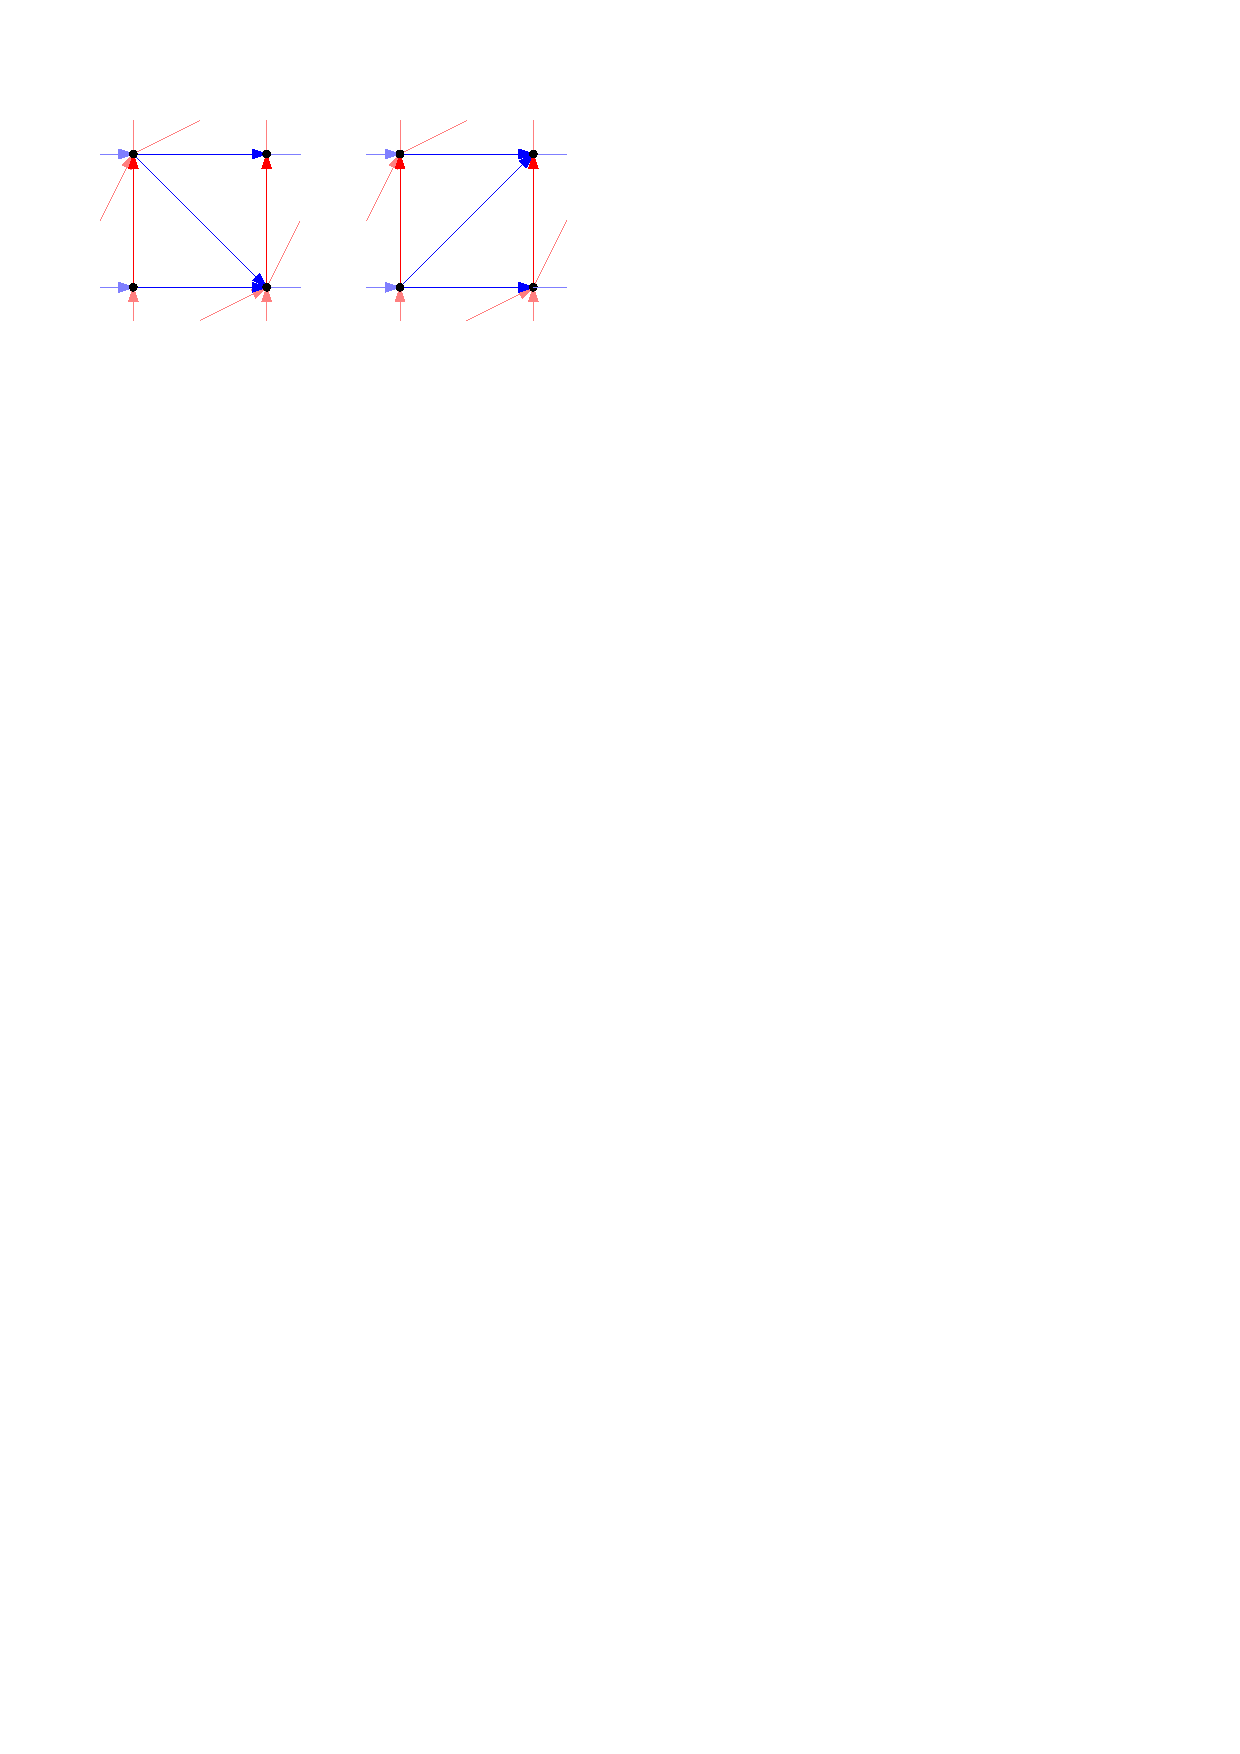
\includegraphics[scale=1]{unifiedAlgo/img/zflip/blueZ.pdf}
    \caption{The two possible blue $Z$'s.}
    \label{fig:zflip:blueZ}
    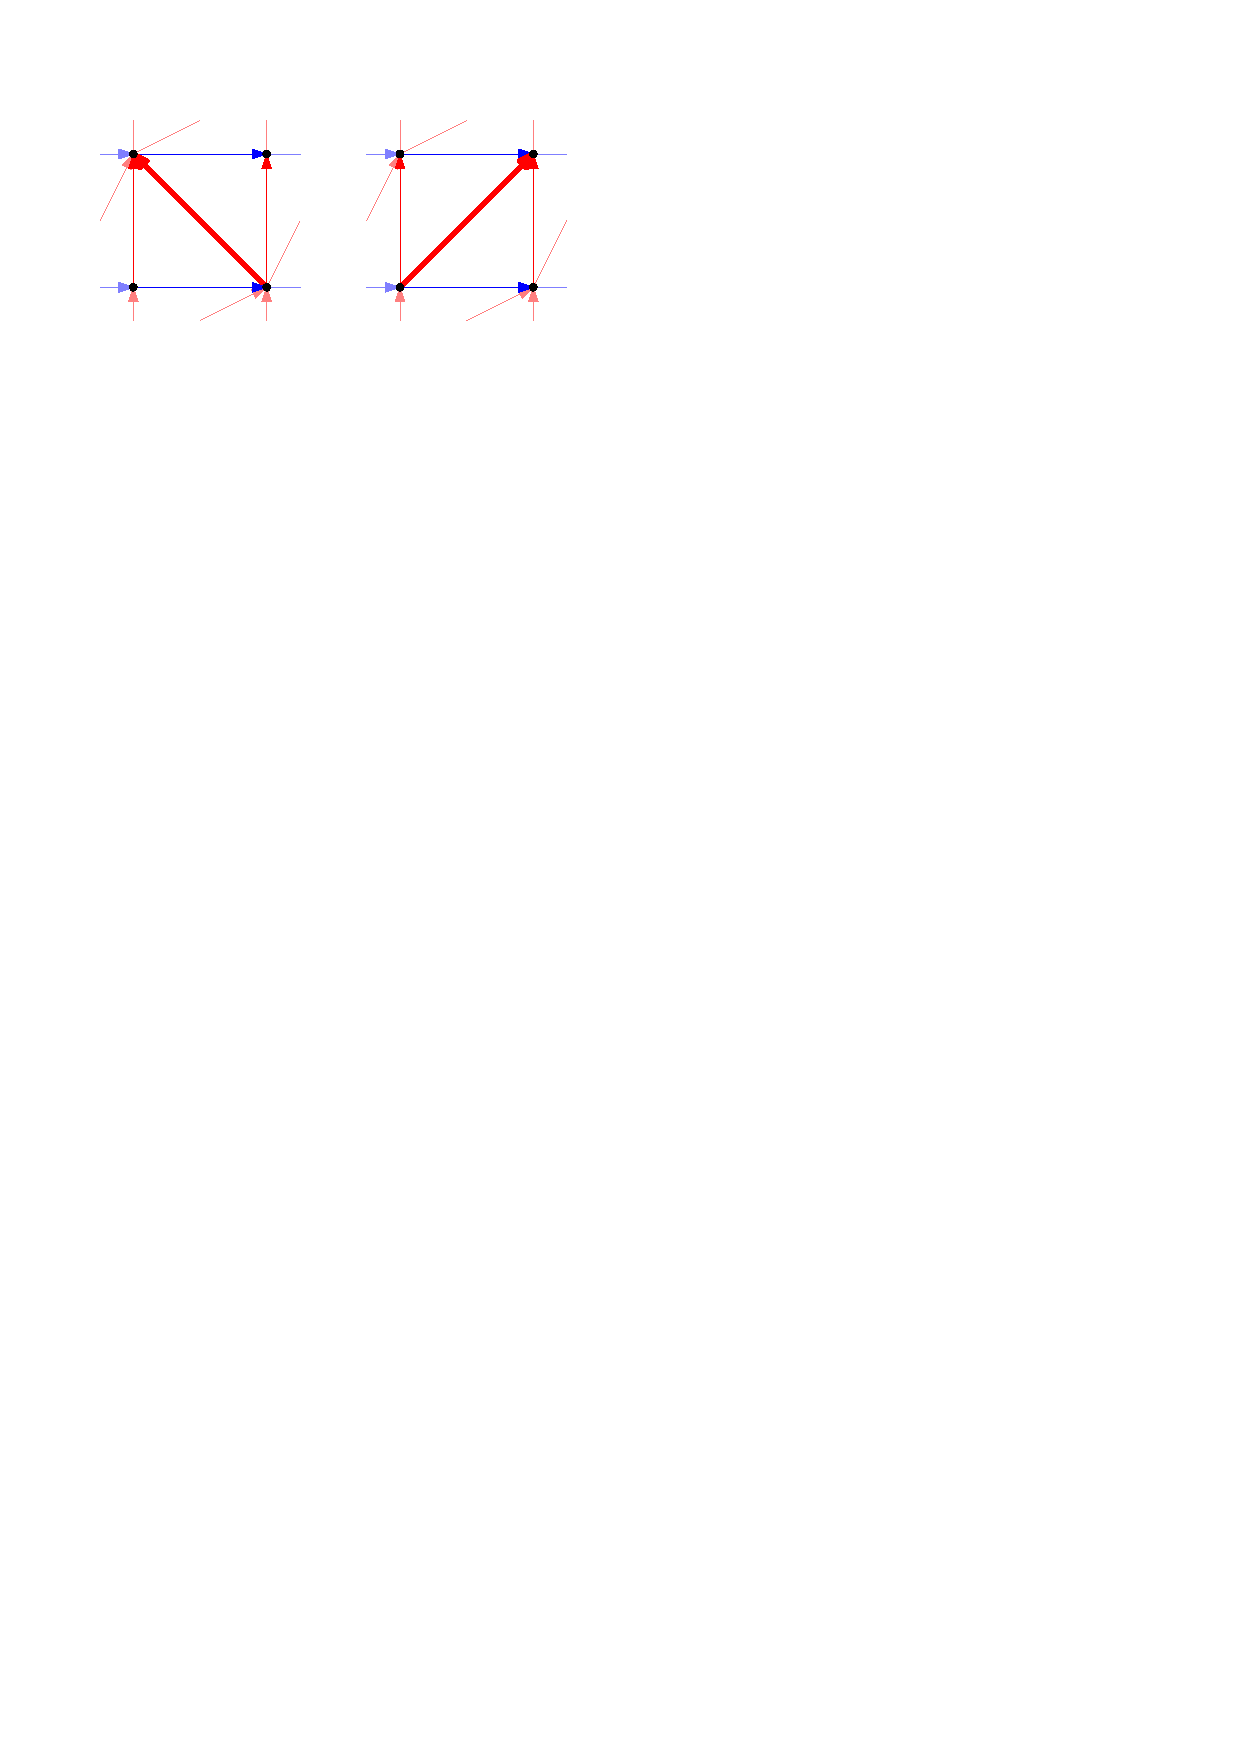
\includegraphics[scale=1]{unifiedAlgo/img/zflip/flip.pdf}
    \caption{The flip.}
    \label{fig:zflip:flip}
  \end{figure}

  As long as the regular edge labeling is not vertically one-sided we find such a blue $Z$ and recolor its middle edge as in Figure~\ref{fig:zflip:flip}. We call this a \emph{flip} and we will say that this edge is \emph{flipped}.
  Note that both flips transfer a valid regular edge labeling to another valid regular edge labeling. If the interior vertex condition was fulfilled in Figure~\ref{fig:zflip:blueZ}, then it is also fulfilled in Figure~\ref{fig:zflip:flip}.

  We repeat these flips until the regular edge labeling is vertically one-sided.
  Since every flip reduces the number of blue edges by one, this is a finite procedure.


  \begin{lemma}
    \label{lm:sweep:vertOnsided}
    The result is a vertically one-sided rectangular edge labeling.
  \end{lemma}
  \begin{proof}
    We still have a regular edge labeling since the flips maintain a regular edge labeling.
    By construction, we flip all blue $Z$'s. If we do not have anymore $Z$'s, then the remaining regular edge labeling is vertically one-sided by Lemma \ref{lm:zflip:blueZNorVertOneSided}.
  \end{proof}

  \begin{lemma}
    \label{lm:zflip:NoTwoSplitsAboveEachOtherVertOnesided}
    Let $v$ be any splitvertex. Then the subsequent vertex on the bottom path $w$ can not be the handle of a large topfan.
  \end{lemma}

  \begin{proof}
    This is the same statement as in Lemma \ref{lm:sweep:NoTwoSplitsAboveEachOther}. We will show that the operation of flipping $Z$'s does not compromise the validity of this statement.

    The flips in this section can only reduce the number of split vertices.
    Hence, it suffices to show that the statement still holds for all previously existing split vertices.

    For a split vertex $v$ adjacent to $\pS$ we can note that the edge $vw$ will not be flipped because it can not be a middle edge.
    Hence, $w$ is still on the bottom path and still not the handle of a big topfan.

    If $v$ is a split vertex due to a chord the edges of $\P$ and $ab$ in Figure~\ref{fig:sweep:botomPathChord} can not have been flipped since then we would find a monochromatic red triangle while a flip leads to another valid regular edge labeling.
    Hence, $w$ is still on the bottom path through $v$ and still can not be the handle of a large topfan.
  \end{proof}
